

\documentclass[../../tc_tp3_main.tex]{subfiles}

\begin{document}
\chapter{Control de tonos y ecualizador de fase}

Un ecualizador es un dispositivo que modifica la ganancia de determinadas frecuencias, de esta manera se altera el contenido de graves, medios y agudos.
\\
Se implementó el siguiente ecualizador, donde K es una constante que vale entre 0 y 1, modelando un potenciómetro.

\begin{figure}[H]
\centering
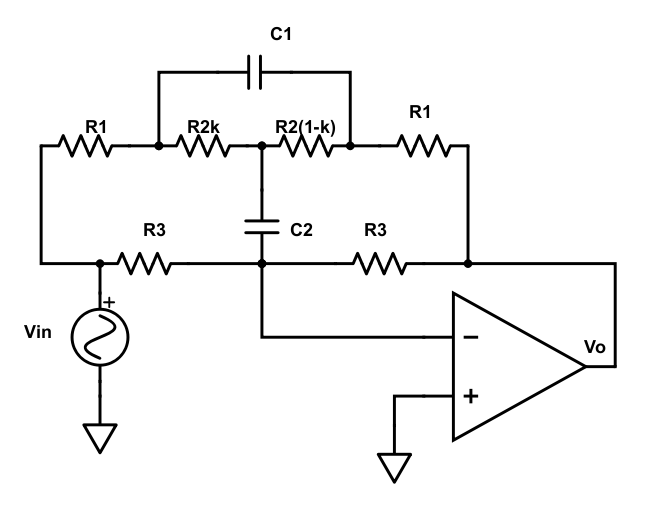
\includegraphics[width=0.45\textwidth]{imagenes/circuitoControlTonos.png}
\caption{Circuito del control de tonos} \label{fig:cct}
\end{figure}




\section{Función transferencia}

Para hallar la función transferencia $H(S)=\frac{V_{o}}{V_{in}} $del circuito de la figura \ref{fig:cct}, se realizaron transformaciones estrella a triangulo y viceversa, reduciendo el circuito. Dichas transformaciones se realizaron con Matlab.



\begin{figure}[H]
\centering
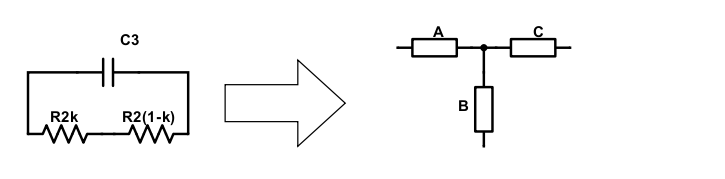
\includegraphics[width=0.5\textwidth]{imagenes/simpl1.png}
\caption{Transformación triangulo a estrella} \label{fig:cs1}
\end{figure}

Reemplazando el circuito triangulo por el estrella, permitio agrupar $A$ con $R_1$, $C$ con$ R_1$ y$ B$ con $C_1$. Obteniendo un nuevo circuito estrella con las siguientes impedancias $ K_1$ , $K_2$ y  $K_3$, tal como se observa en la figura \ref{fig:cs2}.

\begin{gather}
   A=\frac{K\, R_{2}}{C_{1}\, S\, \left(\frac{1}{C_{1}\, S} - R_{2}\, \left(K - 1\right) + K\, R_{2}\right)} \\
B=-\frac{R_{2}\, \left(K - 1\right)}{C_{1}\, S\, \left(\frac{1}{C_{1}\, S} - R_{2}\, \left(K - 1\right) + K\, R_{2}\right)}\\
C=-\frac{K\, {R_{2}}^2\, \left(K - 1\right)}{\frac{1}{C_{1}\, S} - R_{2}\, \left(K - 1\right) + K\, R_{2}}
\end{gather}


\begin{figure}[H]
\centering
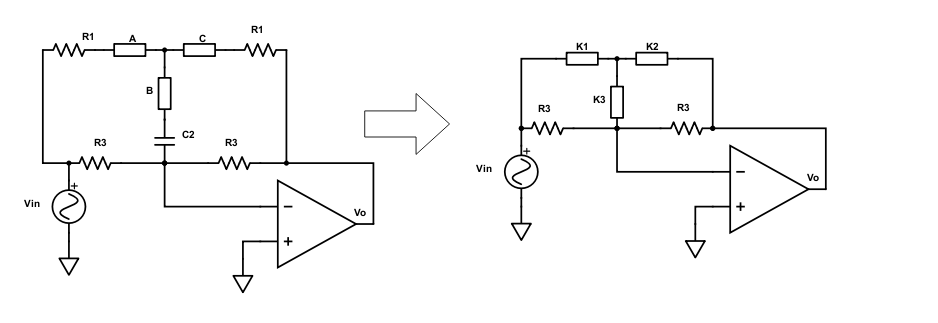
\includegraphics[width=0.5\textwidth]{imagenes/simpl2.png}
\caption{Agrupo impedancias en serie} \label{fig:cs2}
\end{figure}


\begin{figure}[H]
\centering
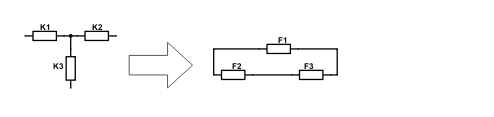
\includegraphics[width=0.5\textwidth]{imagenes/simpl3.png}
\caption{Transformación estrella a triangulo} \label{fig:cs3}
\end{figure}

Dicho circuito estrella se lo transformó a triangulo para de esta manera poder agrupar $F_2$ con $R_3$ y $F_3$ con $R_3$ (figura \ref{fig:cs4}).




\begin{figure}[H]
\centering
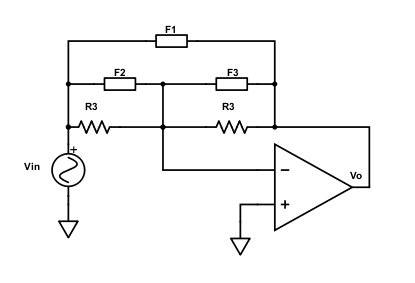
\includegraphics[width=0.5\textwidth]{imagenes/simpl4.png}
\caption{Agrupo impedancias en paralelo} \label{fig:cs4}
\end{figure}



\begin{figure}[H]
\centering
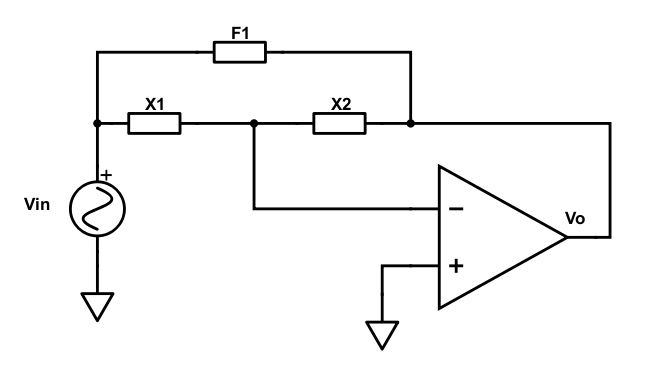
\includegraphics[width=0.5\textwidth]{imagenes/simplFin.png}
\caption{Circuito equivalente} \label{fig:csFin}
\end{figure}

Finalmente se obtiene el circuito de la figura \ref{fig:csFin}. Considerando que el OpAmp se comporta idealmente y la corriente que circula internamente por la entrada del amplificador es cero, resulta la siguiente  función transferencia:

\begin{equation}
H(S)=- \frac{X_2}{X_1}\label{eq:circuitoRed}
\end{equation}

Donde

\begin{gather}
X_1= \frac{1}{\frac{\# 1}{\#3 \# 2 + \#1 \#3 + \# 1 \# 2}+\frac{1}{R_3}}  \\
X_2= \frac{1}{\frac{* 1}{*3 * 2 + *1 *3 + * 1 * 2}+\frac{1}{R_3}} \\
*1=R1 +\frac{KR_2}{C_1 S \left(         \frac{1}{C_1 S} - R_2(K-1)+KR_2                 \right)}\\
*2=\frac{1}{C_2 S} -\frac{KR_2^2 (K-1)}{ \left(         \frac{1}{C_1 S} - R_2(K-1)+KR_2                 \right)}\\
*3=R1 -\frac{KR_2}{C_1 S \left(         \frac{1}{C_1 S} - R_2(K-1)+KR_2                 \right)}\\
\#1=R_1 - \frac{R_2(K-1)}{C_1S \left(  \frac{1}{C_1 S} - R_2 (K-1) + KR_2     \right)}\\
\#2=\frac{1}{C_2 S}- \frac{R_2^2(K-1)K}{ \left(  \frac{1}{C_1 S} - R_2 (K-1) + KR_2     \right)}\\
\#3=R_1 + \frac{R_2K}{C_1 S \left(  \frac{1}{C_1 S} - R_2 (K-1) + KR_2     \right)}
\end{gather}

Aplicando las siguientes condiciones de diseño sobre la función transferencia
\begin{gather}
 R_3 >> R_1   \\
 R_3 =10 R_2   \\
C_1=10C_2
\end{gather}

Obtenemos


\begin{gather}
H(S)=-\frac{AS^2+BS+C}{AS^2+DS+C}\\
\begin{split}
A=-20C_{2}^2 K^2 R_{2}^2 R_{1}   +    20 C_{2}^{2} K R_{1} R_{2}^2 + \\ 10 C_{2}^2 R_{1}^2 R_{2} +  100 C_{2}^{2} R_{1} R_{2}^2  
\end{split}\\
\begin{split}
B= -C_2K^2 R_2^2 -9 C_2 K R_2^2  \\+ C_2 R_1^2  + 31 C_2 R_1 R_2  + 10 C_2 R_2^2  
\end{split}\\
\begin{split}
D=-C_2 K^2 R_2^2+11C_2K R_2^2 +\\ C_2 R_1^2+31 C_2 R_1 R_2
\end{split}\\
C=2R_1+R_2
\end{gather}





Si
\begin{equation}
\begin{split}
-20C_{2}^2 K^2 R_{2}^2 R_{1}  S^{2} +    20 C_{2}^{2} K R_{1} R_{2}^2+\\ 10 C_{2}^2 R_{1}^2 R_{2} S^{2} + 100 C_{2}^{2} R_{1} R_{2}^2 S^{2}  \\   \approx 100 C_{2}^2 R_{1} R_{2} ^2 S^2
\end{split}
\end{equation}

\begin{gather}
H(S)=-\frac{AS^2+BS+C}{AS^2+DS+C} \label{eq:MfinalR}\\
\begin{split}
A=100 C_{2}^2 R_{1} R_{2} ^2 S^2
\end{split}\\
\begin{split}
B= -C_2K^2 R_2^2 -9 C_2 K R_2^2  \\+ C_2 R_1^2  + 31 C_2 R_1 R_2  + 10 C_2 R_2^2  
\end{split}\\
\begin{split}
D=-C_2 K^2 R_2^2+11C_2K R_2^2 + \\ C_2 R_1^2+31 C_2 R_1 R_2
\end{split}\\
C=2R_1+R_2
\end{gather}

La ecuacion \ref{eq:MfinalR} posee la forma

\begin{equation}
H(S)=\frac {\left( \frac{S}{W_0} \right) ^2 + \frac{S}{Q_Z W_0} +1}{\left( \frac{S}{W_0} \right) ^2 +\frac{S}{Q_Z W_0}+1} \label{eq:MpasaBanda}
\end{equation}
Dicha función transferencia corresponde a un circuito pasa banda de segundo orden, donde $W_0$ es la frecuencia central de la banda y $Q_Z$ , $Q_P$, son los respectivos factores de calidad.
\subsection{Frecuencia central}
El coeficiente normalizado del término $S^2$, tanto para el numerado como en el denominador (ecuación zz), es:
\begin{equation}
\frac{100 C_{2}^2 R_{1} R_{2} ^2}{2R_1+R_2}  \label{eq:coefP}
\end{equation}
Entonces por la ecuación \ref{eq:MpasaBanda} y \ref{eq:coefP}, se obtiene la frecuencias central del pasa banda.

\begin{gather}
W_0^2=\frac{1}{ecuacion \ref{eq:coefP}}=\frac{2R_1+R_2}{100 C_{2}^2 R_{1} R_{2} ^2}   \\
W_0=\frac{\sqrt{2+\frac{R_2}{R_1}}}{10C_2 R_2}\\
f_0=\frac{\sqrt{2+\frac{R_2}{R_1}}}{20 \pi C_2 R_2} \label{eq:MfrecCen}
\end{gather}
\subsection{Factores de calidad}
A partir de los coeficientes normalizados de los términos de S, obtenemos los factores de calidad




\subsubsection{Factor de calidad $Q_Z$}
El coeficiente normalizado correspondiente al termino de $S$ del numerador, es
\begin{equation}
\frac{-C_2 K ^2 R_2^2 - 9  C_2 K R_2 ^2 + C_2 R_1^2 +31 C_2 R_1 R_2+10 C_2 R_2^2}{2R_1 +R_2} \label{eq:coefNUM}
\end{equation}


Entonces por la ecuación \ref{eq:MpasaBanda} y \ref{eq:coefNUM}, se obtiene:

\begin{gather}
Q_Z=\frac{1}{W_0 \cdot ecuacion\ref{eq:coefNUM}}\\
Q_Z=\frac{\left( 2R_1 +R_2 \right) 10 R_2 }{\left( - K ^2 R_2^2 - 9   K R_2 ^2 +  R_1^2 +31  R_1 R_2+10  R_2^2 \right)\sqrt{2+\frac{R_2}{R_1}} }
\end{gather}







\subsubsection{Factor de calidad $Q_P$}
El coeficiente normalizado correspondiente al termino de $S$ del denominador, es
\begin{equation}
\frac{-C_2 K ^2 R_2^2 + 11  C_2 K R_2 ^2 + C_2 R_1^2 +31 C_2 R_1 R_2}{2R_1 +R_2} \label{eq:coefDEN}
\end{equation}


Entonces por la ecuación \ref{eq:MpasaBanda} y \ref{eq:coefDEN}, se obtiene:

\begin{gather}
Q_P=\frac{1}{W_0 \cdot ecuacion\ref{eq:coefDEN}}\\
Q_P=\frac{\left( 2R_1 +R_2 \right) 10 R_2 }{\left( - K ^2 R_2^2 + 11   K R_2 ^2 +  R_1^2 +31  R_1 R_2 \right)\sqrt{2+\frac{R_2}{R_1}} }
\end{gather}


\subsubsection{Modulo de $H(f)$ en $W_0$}
Definimos $A_0$ como:
\begin{equation}
A_0	\widehat{=} \mid H(S=jW_0) \mid
\end{equation}

Reemplazamos $S=jW_0$ en \ref{eq:MpasaBanda}

\begin{gather}
A_0 =\frac{Q_P}{Q_Z}\\
A_0=\frac{- K ^2 R_2^2 - 9   K R_2 ^2 +  R_1^2 +31  R_1 R_2+10  R_2^2}{ - K ^2 R_2^2 + 11   K R_2 ^2 +  R_1^2 +31  R_1 R_2 }
\end{gather}
Si $K=0$

\begin{equation}
\begin{split}
A_0(K=0) =\frac{R_1^2 +31  R_1 R_2+10  R_2^2}{  R_1^2 +31  R_1 R_2}\\
= \frac{R_1(R_1+31R_2)+10R_2^2}{R_1(R_1+31R_2)}\\
\approx \frac{R_1 31 + 10 R_2}{31 R_1}
\end{split}
\end{equation}
\begin{equation}
A_0(K=0) \approx \frac {3R_1 + R_2}{3R_1} \label{eq:A00}
\end{equation}

Si $K=1$

\begin{equation}
\begin{split}
A_0(K=1) =\frac{R_1^2 + 31R_1 R_2}{10 R_2^2 +R_1^2+31R_1 R_2} \\
\approx \frac{R_1 31}{10 R_2 + 31 R_1} \\
 \approx \frac{3 R_1}{R_2 + 3 R_1}
\end{split}
\end{equation}

\begin{equation}
A_0(K=1) \approx \frac {3R_1}{3R_1 + R_2}\label{eq:A01}
\end{equation}

A partir de \ref{eq:A00} y \ref{eq:A01} obtenemos que

\begin{equation}
\frac {3R_1}{3R_1 + R_2} \leq A_0  \leq \frac{3R_1 + R_2}{3R_1}\label{eq:rangoA}
\end{equation}



\section{Análisis paramétrico}


La función transferencia depende de un parámetro K que pertenece al intervalo 0,1. Dicho parámetro provino del modelado del potenciómetro. Para analizar el funcionamiento del circuito, se realizaron gráficos de las distintas características del circuito en función de la constante.

\begin{figure}[H]
\centering
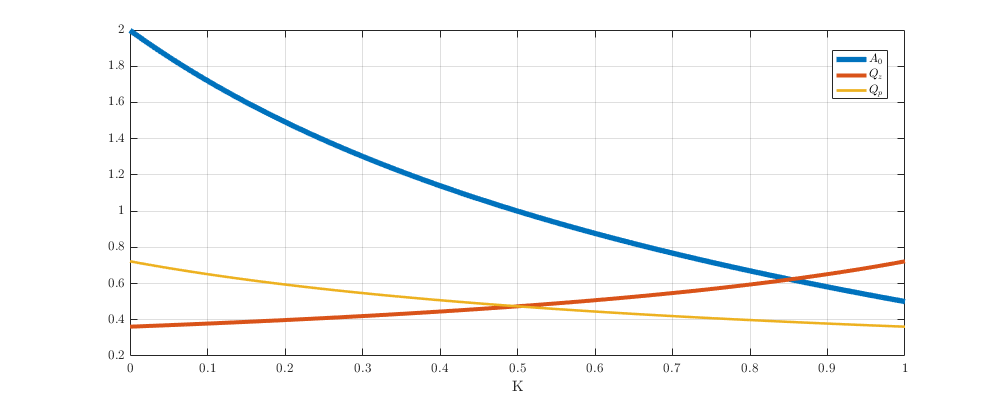
\includegraphics[width=0.55\textwidth]{imagenes/param.png}
\caption{Diagrama parametrico} 
\end{figure}

Como se observa en la figura, la posición del potenciómetro altera la ganancia del circuito (linea azul), con k=0 el circuito multiplica la entrada por 2(gana 6dB) y con K=1 multiplica a la entrada por 0.5 (atenúa 6dB).



\begin{figure}[H]
\centering
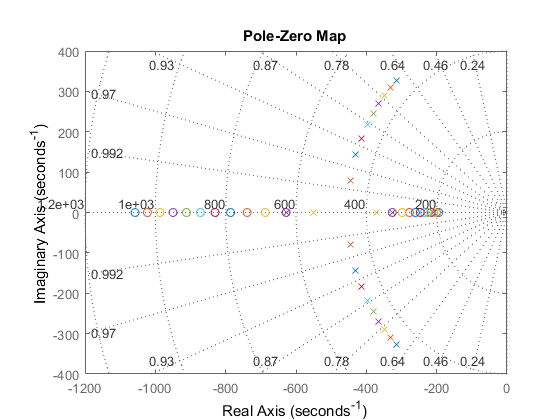
\includegraphics[width=0.55\textwidth]{imagenes/param005.png}
\caption{Diagrama parametrico- polos y ceros -  k desde 0 a 0.5} 
\end{figure}

k variando desde cero a 0.5, se observa que los ceros son reales y ce aproximan hacia el valor de $-w_0$ en el eje real. En cuanto a los polos se alejan del eje imaginario. 


\begin{figure}[H]
\centering
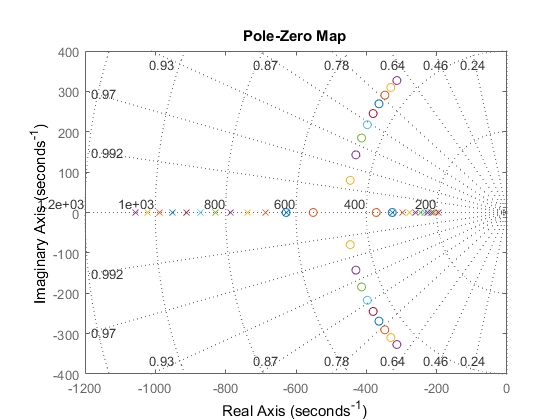
\includegraphics[width=0.55\textwidth]{imagenes/param051.png}
\caption{Diagrama parametrico- polos y ceros -  k desde 0.5 a 1} 
\end{figure}


k variando desde 0.5 a 1, se observa que los polos son reales y que a medida que aumenta k se alejan del valor de $-w_0$. Los ceros son imaginarios y a medida que aumenta k se acercan al eje imaginario.


\begin{figure}[H]
\centering
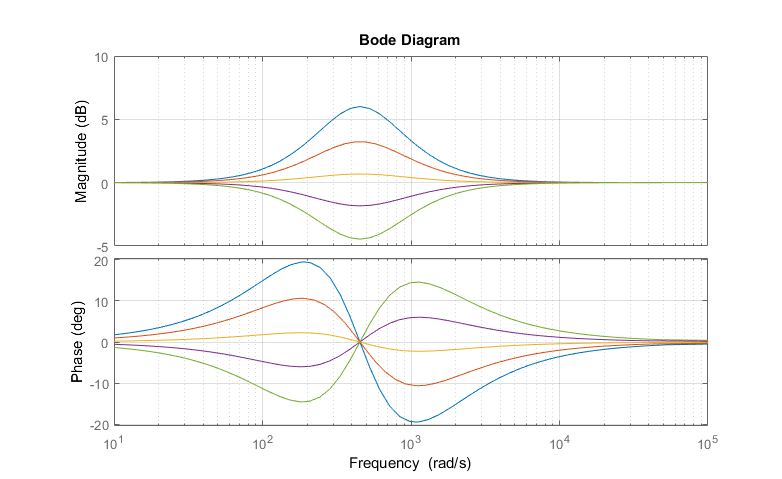
\includegraphics[width=0.55\textwidth]{imagenes/paramBode.png}
\caption{Diagrama parametrico- respuesta en frecuencia} 
\end{figure}

Como se observa en el gráfico de la respuesta en frecuencia, cuando k vale 0 se produce la máxima ganancia y a medida que aumenta disminuye la ganancia hasta el punto de no atenuar ni ganar (k=0.5) y a partir de ese punto comienza a atenuar.

\section{Análisis de singularidades}

Partiendo de que el comportamiento del circuito es descripto por la ecuación \ref{eq:MpasaBanda} , y que $Q_p$ se rfiere al factor de calidad de los polos, $Q_z$ se refiere al factor de calidad de los ceros y $W_0$ es la frecuencia de pasa banda.
\subsection{Polos}
Aplicando la formula resolvente obtenemos:
$$Polos_{1,2}=-\frac{W_0}{2 Q_p} \pm \frac{W_0}{2}\sqrt{\frac{1}{Q_p^2}-4}$$
Como Qp siempre es positivo para todo valor de r1,r2 , c2 y k entre 0 y 1. Entonces la parte real de los polos siempre es negativa, Por ende el sistema es estable. Además los polos  tienen parte imaginaria no nula son polos conjugados
\subsection{Ceros}
El resultado de aplicar la formula resolvente:
$$Ceros_{1,2}=-\frac{W_0}{2 Q_z} \pm \frac{W_0}{2}\sqrt{\frac{1}{Q_z^2}-4}$$
Análogamente a los polos, también se cumple que Qz sea positivo. Por ende, la parte real de los ceros es negativa y son complejos conjugados.

\subsection{Sistema de fase mínima}

Se definen los sistemas de fase mínima, como aquellos que sus singularidades se encuentren en el semiplano izquierdo. 
\\
Como se mostró anteriormente, tanto los polos y ceros se encuentran en el semiplano izquierdo, por ende el sistema es de fase mínima.

\section{Ecualizador de fase}

Un ecualizador de fase es un circuito que no altera la amplitud de la señal pero si la fase.
Se desea implementar un circuito de segundo orden, que pueda convertir un sistema de fase mínima a uno de fase no mínima.
\\
Se implementó el siguiente circuito:
\begin{figure}[H]
\centering
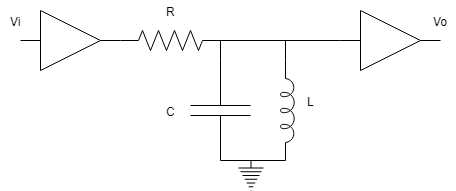
\includegraphics[width=0.35\textwidth]{imagenes/eqFase.png}
\caption{Ecualizador de fase - circuito} 
\end{figure}

Aplicando la formula de divisor de tension se obtiene la funsion transferencia:

\begin{equation}
H(S)=\frac{L}{R}\frac{S}{\frac{S^2}{\frac{1}{LC}}+\frac{SL}{R} +1}\label{eq:eqFase}
\end{equation}

Tal como se observa en la función transferencia, los polos poseen su parte real negativa (por ende el sistema es estable). En cuanto al cero, este se encuentra en el origen entonces el sistema no es de fase mínima.
\\
Para hallar la función transferencia final, basta con multiplicar \ref{eq:eqFase} y \ref{eq:MfinalR}.
\todo{ver que hicieron los demas}















\section{Equalizador de 3 bandas}

\subsection{Espectro audible}
Los seres humanos, pueden percibir un rango de frecuencias, desde 20Hz hasta 20KHz. Dicho rango depende de la salud auditiva de cada persona.
\\ El espectro se puede dividir en tres partes, llamadas graves, medios y agudos.

\begin{itemize}
  \item Tonos graves, frecuencias comprendidas entre 20Hz y 256Hz.
  \item Tonos medios, frecuencias comprendidas entre 256Hz y 2KHz.
  \item Tonos Agudos, frecuencias comprendidas entre 2KHz y 20KHz.
\end{itemize}
\subsection{Elección de la frecuencia central}

Como se trata de un ecualizador de tres bandas, se deben elegir una frecuencia central para cada  pasa banda. Consideramos que las frecuencias deben estar equiespaciadas en escala logarítmica, para lograr abarcar todo el espectro audible.
Para ello utilizamos la media geométrica,$fo=\sqrt{f_{inicial}f_{final}}$. De esta manera calculamos las frecuencias de cada banda, representando los tonos grabes, medios y agudos.
\begin{table}[h]
\begin{center}
\begin{tabular}{|l|l|l|}
\hline
Etapa & Tonos & $f_0$ \\
\hline \hline
1&Graves  &64Hz \\ \hline
2&Medios  &716Hz \\ \hline
1&Agudos  &6324Hz \\ \hline

\end{tabular}
\caption{Frecuencias centrales} 
\label{tab:MFc}
\end{center}
\end{table}

\subsection{Ganancia en la frecuencia central - $A_0$}

Los ecualizadores comerciales se construyen de 3 ganancias/atenuaciones en las frecuencias centrales de cada banda, de 6dB, 12dB y 18dB.
\\En este caso elegimos que nuestro ecualizador atenué o amplifique 6dB, para así evitar que el amplificador operacional sature.
\\
\\Reemplazando el criterio de los 6dB en \ref{eq:rangoA}

\begin{gather}
 \frac{3R_1 + R_2}{3R_1}=2\\
\frac {3R_1}{3R_1 + R_2} =0.5
\end{gather}

Resolviendo el sistema de ecuaciones obtenemos
\begin{equation}
R_2=3R_1 \label{eq:Mrelacionr}
\end{equation}

Reemplazando \ref{eq:Mrelacionr} en \ref{eq:MfrecCen} y despejando, obtenemos una expresion para hallar $C_2$

\begin{equation}
C_2=\frac{\sqrt{5}}{20 \pi R_2 f_0}
\end{equation}


A partir de este resultado, de las frecuencias de corte y de las condiciones de diseño ya mencionadas, se calcularon los componentes de cada etapa.

\begin{table}[h]
\begin{center}
\begin{tabular}{|l|l|l|l|l|l|l|}
\hline
Etapa & $R_1$ & $R_2$ & $R_3$ & $C_1$ & $C_2$ & $f_0$  \\
\hline \hline
1& 1.6$K \Omega$ & 5$K \Omega$   & 50$K \Omega$ & 1\micro F & 100$n$F & 71Hz\\ \hline
2& 1.6$K \Omega$ & 5$K \Omega$   & 50$K \Omega$ & 100$n$F & 10$n$F & 776Hz\\ \hline
3& 1.6$K \Omega$ & 5$K \Omega$   & 50$K \Omega$ &12$n$F & 1.2$n$F &6000Hz\\ \hline


\end{tabular}
\caption{Compoenentes} 
\label{tab:MComponentes}
\end{center}
\end{table}

\subsection{Conexión de las etapas}
Las etapas se podrían conectar de dos maneras, en cascada o en paralelo.
\subsubsection{Cascada}
La salida de una etapa se conecta a la entrada de la otra etapa. Si $H_1$, $H_2$ y $H_3$, son las funciones transferencia de cada etapa,entonces  la función transferencia del sistema es $H=H_1 H_2 H_3$.

\begin{figure}[H]
\centering

\includegraphics[width=0.5\textwidth]{imagenes/cascada.png}
\caption{Esquema de conexion cascada} 
\end{figure}

\subsubsection{Paralelo}
Las entradas de cada etapa se conectan juntas y las salidas también. Sin embargo las salidas se deben conectar juntas a través de por ejemplo un sumador.
\\En esta configuración la función transferencia del sistema es $H=H_1+ H_2+ H_3$.

\begin{figure}[H]
\centering
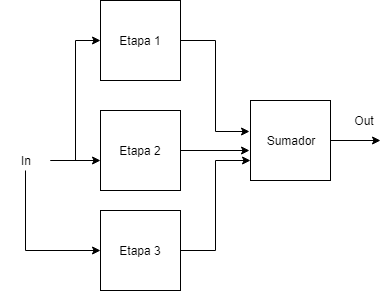
\includegraphics[width=0.5\textwidth]{imagenes/paralelo.png}
\caption{Esquema de conexion paralelo} 
\end{figure}


\subsubsection{Simulación}
Se simularon ambas configuraciones cascada y paralelo.

\begin{figure}[H]
\centering
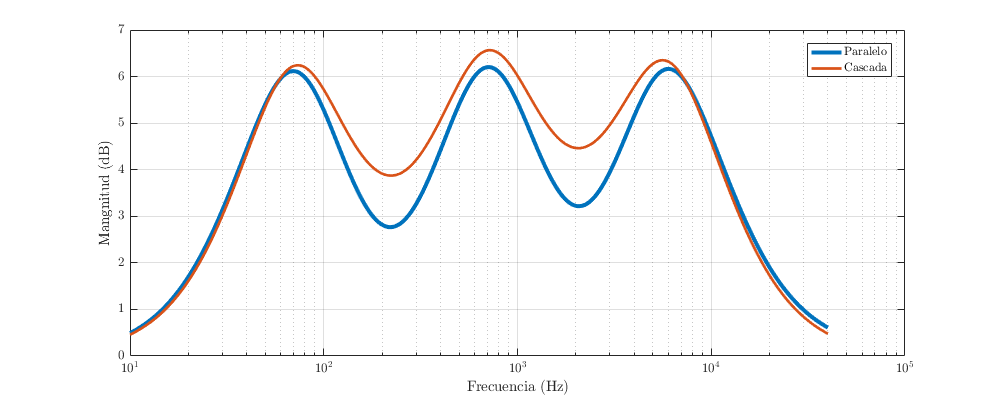
\includegraphics[width=0.55\textwidth]{imagenes/parCasSimMax_m.png}
\caption{Maxima ganancia - magnitud} 
\end{figure}

\begin{figure}[H]
\centering
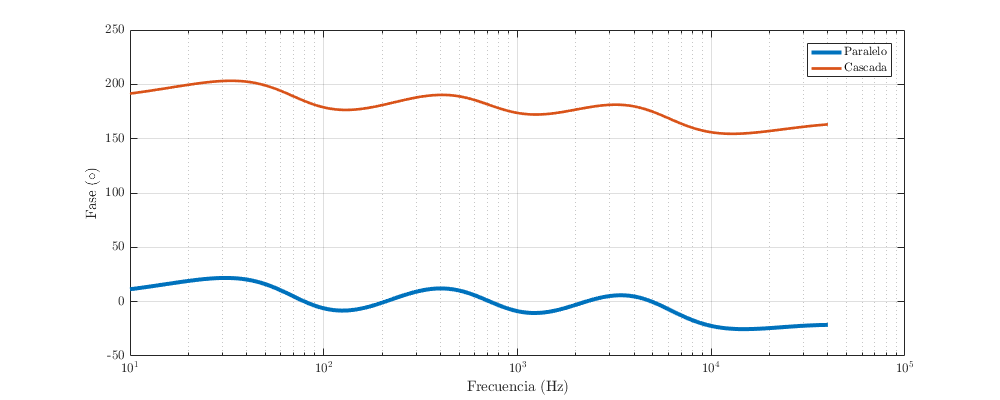
\includegraphics[width=0.55\textwidth]{imagenes/parCasSimMax_f.png}
\caption{Maxima ganancia - fase} 
\end{figure}

\begin{figure}[H]
\centering
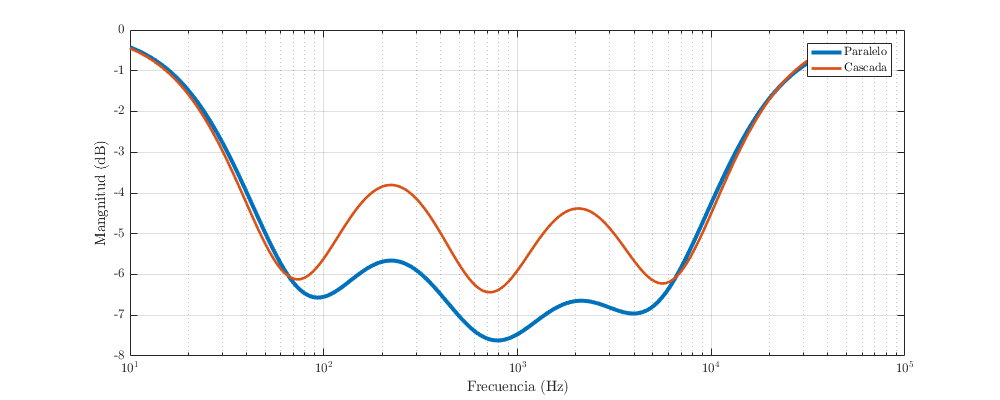
\includegraphics[width=0.55\textwidth]{imagenes/parCasSimMin_m.png}
\caption{Maxima atenuación - magnitud} 
\end{figure}

\begin{figure}[H]
\centering
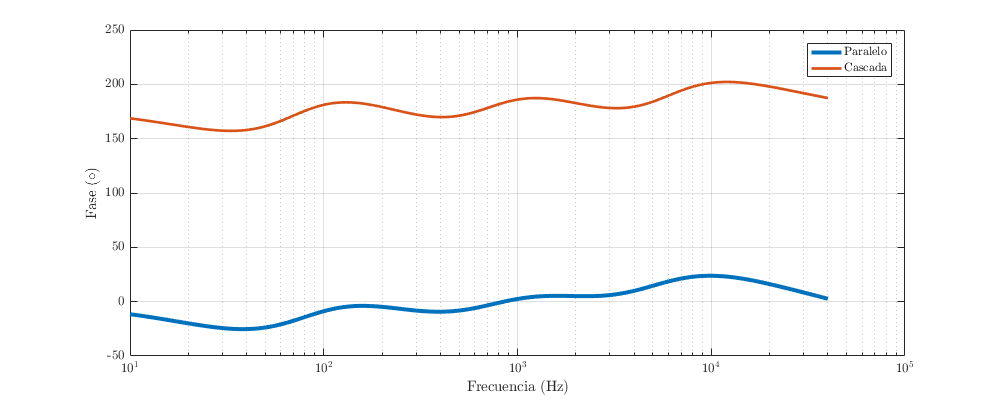
\includegraphics[width=0.55\textwidth]{imagenes/parCasSimMin_f.png}
\caption{Maxima atenuación - fase} 
\end{figure}

Como se observa en los gráficos, en la condición de máxima ganancia la amplitud de los sobre picos es mayor en paralelo y en máxima atenuación la máxima atenuación de los sobre picos corresponde a la configuración cascada.


\subsubsection{Just-noticeable difference (JND)}
Es al minima cantidad de algo que el humano puede persicir, por lo menos en la mtidad de los casos. En el caso del audio, la minama variacion perceptible es de 1dB.
\subsubsection{Figura de ruido}
\todo{mejorar lo del ruido}
El objetivo es determinar que configuración que es más susceptible al ruido. Los componentes, tantos pasivos como activos generan ruido. En  la conexión cascada el ruido de cada etapa es amplificado por la etapa posterior, por ende posee más ruido que la configuración en paralelo.

\subsubsection{Elección de topología}

En cuanto al JND tanto el paralelo como  serie, dependiendo si se encuentra en máxima ganancia o atenuación, tienen máxima amplitud, por ende no es criterio para elegir. El oído humano no puede percibir la diferencia de fase, por lo tanto no aporta a la elección de topología.
\\Sobre el ruido, la configuración paralelo, tiene una leve ventaja sobre la cascada, sin embargo para realizarla se debe agregar un sumador, lo que complejiza el circuito. Por ende se eligió la topología cascada.

\subsection{Realizacion de la placa}

Se conectaron las tres etapas en cascada, se agregó una entrada de audio mono (Jack 3,5 mini plug) además de pines, también esto se hizo a la salida. En cuanto al amplificador operacional, se decidió utilizar tres Tl081, debido a sus altas prestación en cuanto al slew rate, y ruido.

\subsection{Mediciones}
Se realizaron las siguientes mediciones al circuito:
\begin{itemize}
 \item Respuesta en frecuencia a máxima ganancia.
 \item Respuesta en frecuencia a máxima atenuación.
 \item Respuesta en frecuencia si atenuar o ganar.
 \item Impedancia de entrada máxima y mínima.
 \item Impedancia de salida máxima y mínima.
\end{itemize}

\begin{figure}[H]
\centering
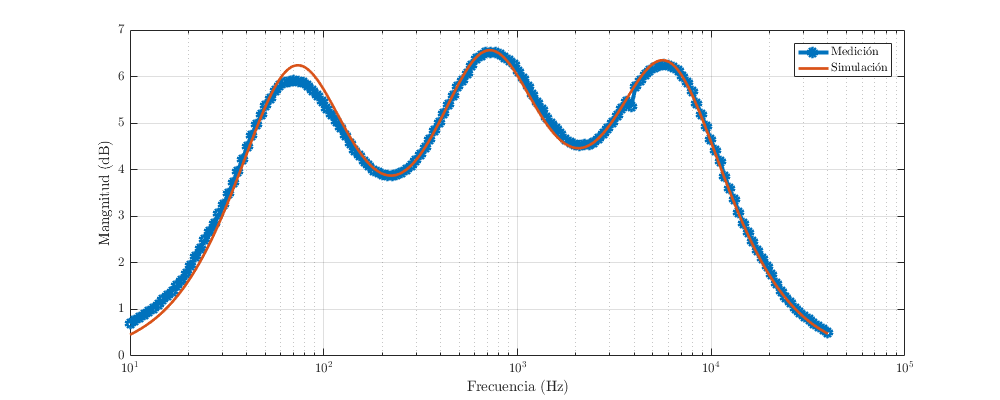
\includegraphics[width=0.55\textwidth]{imagenes/max_m.png}
\caption{Maxima ganancia - magnitud} 
\end{figure}

\begin{figure}[H]
\centering
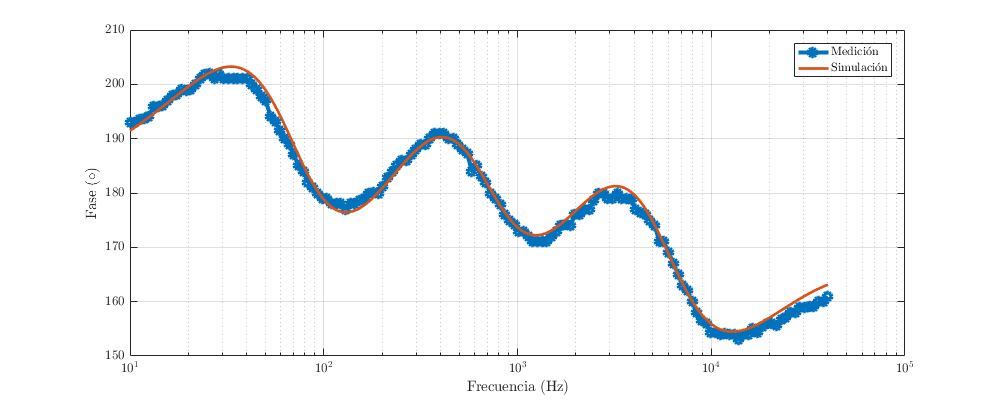
\includegraphics[width=0.55\textwidth]{imagenes/max_f.png}
\caption{Maxima ganancia - fase} 
\end{figure}

\begin{figure}[H]
\centering
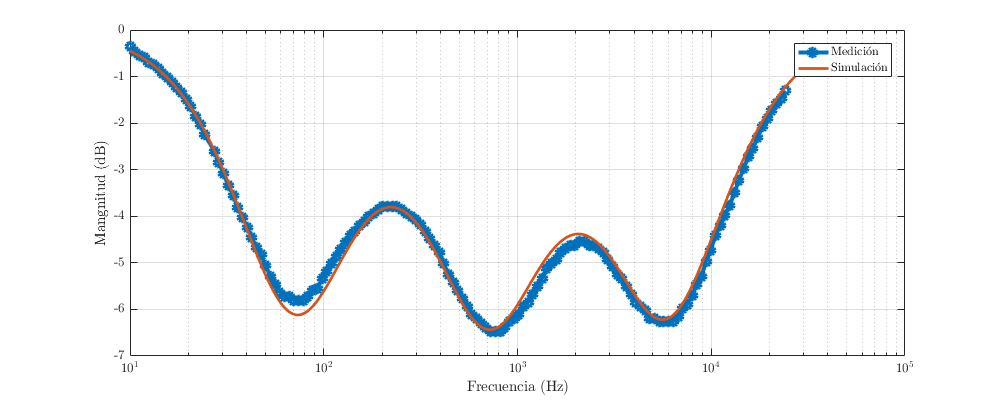
\includegraphics[width=0.55\textwidth]{imagenes/min_m.png}
\caption{Maxima atenuación - magnitud} 
\end{figure}

\begin{figure}[H]
\centering
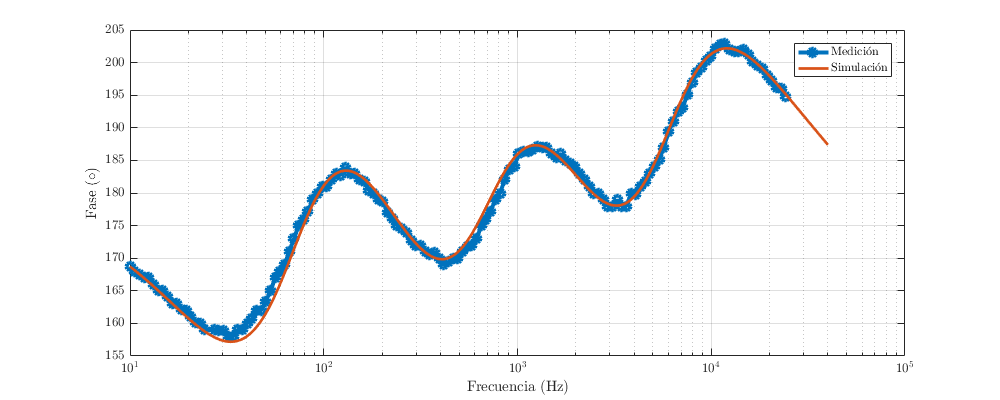
\includegraphics[width=0.55\textwidth]{imagenes/min_f.png}
\caption{Maxima atenuación - fase} 
\end{figure}

\begin{figure}[H]
\centering
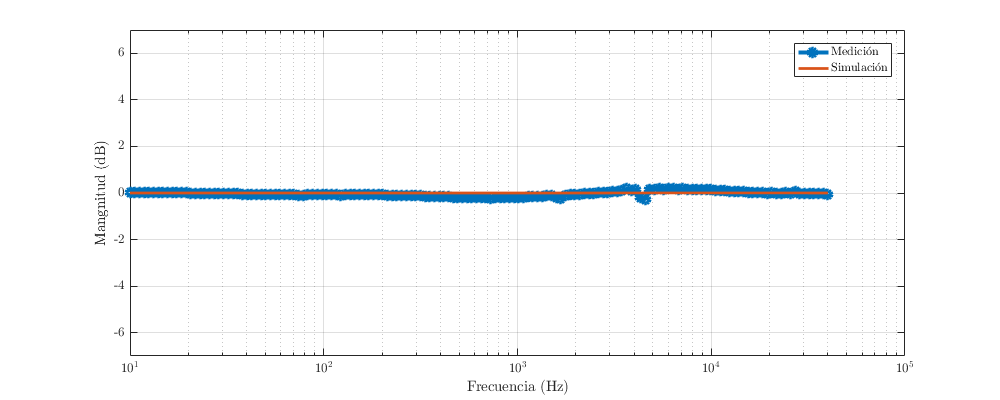
\includegraphics[width=0.55\textwidth]{imagenes/med_m.png}
\caption{Sin ganancia ni atenuación - magnitud} 
\end{figure}

\begin{figure}[H]
\centering
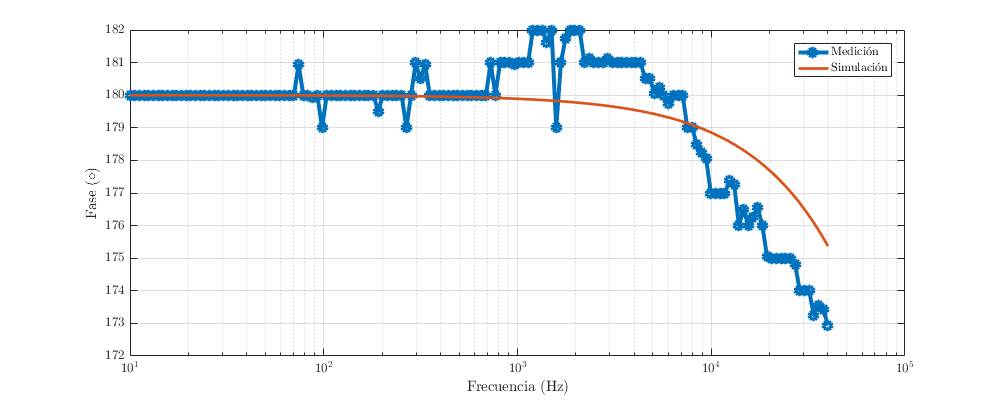
\includegraphics[width=0.55\textwidth]{imagenes/med_f.png}
\caption{Sin ganancia ni atenuación - fase} 
\end{figure}

\begin{table}[h]
\begin{center}
\begin{tabular}{|l|l|l|}
\hline
Impedancia & Maxima & Minima \\
\hline \hline
Entrada& 3.69 $K \Omega$  &1.584 $K \Omega$ \\ \hline
Salida&8.122$\Omega$  &0.022$\Omega$  \\ \hline


\end{tabular}
\caption{Impedancia} 
\label{tab:MImp}
\end{center}
\end{table}
\section{Conclusión}
Se logró realizar el ecualizador de tres bandas, dicho circuito se comportó como era de esperarse en el rango de frecuencias audibles. Tal como se observan en las mediciones, las simulación y las mediciones ajustan perfectamente.



\end{document}
